In a typical instance of the current state of the art algorithm, the
Infinite Impulse Response (IIR), the expansion depends upon the
last ten elements in the input signal history~\cite{Chen:04a}. To make a
fair comparison between fractional derivative or integral algorithms,
it we examine the average Gr{\"u}nwald algorithm with ten bins of input
signal history, such that the history memory requirement is the
same. Figure~\ref{fig:bode10p05} contains a bode plot for a fractional
derivative of order $\alpha=0.5$ with ten history registers. Compared
to the IIR10, the average Gr{\"u}nwald with an exponential binning
structure (EXP10) has approximately a factor of three gain in
constant-phase bandwidth with a ten degree variation allowance. 

The performance of the average Gr{\"u}nwald algorithm improves
dramatically with a small increase in the number of input signal
history bins. Computational limitations were the driving reason behind the choice of the maximal number of input history registers. It was not feasible to run the simulation for more than $10^6$ time steps due to limitations in phase and amplitude reconstruction.  Since the exponential binning structure (EXP) scales most rapidly with history depth, it set the limit on the number of bins that would fill during this number of time steps. Since $\log_2(10^6)\approx 20$, $20$ bins of input signal history were included for all average Gr{\"u}nwald binning structures. Figures~\ref{fig:bode20p05} through~\ref{fig:bode20m05} compare $20$
history memory registers of the IIR to $20$ history memory
registers of the average Gr{\"u}nwald, for a variety of binning
strategies. For both fractional
derivatives and integrals there is a gain in the constant phase
bandwidth of $2$ to $2.5$ decades with a variation of ten degrees allowed.

The specific limitations encountered in generating Figures~\ref{fig:bode20p05} through~\ref{fig:bode20m05} would not be present during runtime on a microcontroller unit (mcu) because there would be no need to store and manipulate the entire past output signal history. However, other limitations might be encountered. We found that it became difficult to initialize the weights in finite time for more than $26$ bins, for instance. Some less well motivated partitioning schemes (not reported here) appeared to go numerically unstable at a lower number of bins, as well. 

\begin{figure}
\epsfig{file=FIG4.eps, height=130mm, width=90mm}
\caption{Magnitude and phase as a function of frequency for 10
  registers of binned (SQ10, EXP10, FIB10) or unbinned (GL10, IIR10)
  input signal history. GL is the full Gr{\"u}nwald calculation, for the
  entire input signal history prior to that time. For this figure, the duration was $10.0$ s, $N_t=10^4$, and $\delta t = 10^{-3}$ s.}
\label{fig:bode10p05}
\end{figure}

\begin{figure}
\epsfig{file=FIG5.eps,height=130mm,width=90mm}
\caption{Bode plots for $20$ bins of input signal memory for $\alpha=0.5$. The duration was $10.0$ s, $N_t=10^6$, and $\delta t = 10^{-5}$ s.}
\label{fig:bode20p05}
\end{figure}

\begin{figure}
\epsfig{file=FIG6.eps,height=130mm,width=90mm}

\caption{Bode plots for $20$ bins of input signal memory for $\alpha=0.3$. The duration was $10.0$ s, $N_t=10^6$, and $\delta t = 10^{-5}$ s. }
\label{fig:bode20p03}
\end{figure}

\begin{figure}
\epsfig{file=FIG7.eps,height=130mm,width=90mm}

\caption{Bode plots for $20$ bins of input signal memory for $\alpha=-0.3$. The duration was $10.0$ s, $N_t=10^6$, and $\delta t = 10^{-5}$ s. }
\label{fig:bode20m03}
\end{figure}

\begin{figure}
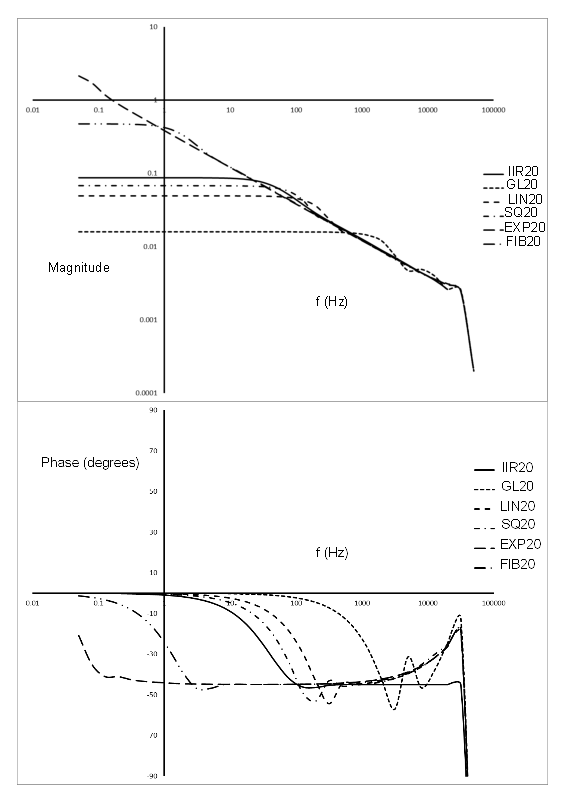
\epsfig{file=FIG8.eps,height=130mm,width=90mm}
\caption{Bode plots for $20$ bins of input signal memory for $\alpha=-0.5$. The duration was $10.0$ s, $N_t=10^6$, and $\delta t = 10^{-5}$ s. }
\label{fig:bode20m05}
\end{figure}